\newpage
\hypertarget{multiEAP}{}
\subsection{Importing and working with multiple EAPs}
\visHeader

Please note that the following instructions on how to properly export and import Enterprise Architect (EA) files is \emph{not} an eMoflon-exclusive feature!
Instead of simply referring you to their instructions, we have included them here as importing projects into the \emph{same} workspace is crucial for
transformations to work.

\begin{itemize}

\item[$\blacktriangleright$] Open the folder where you extracted the contents of the \texttt{Part4.zip} download and open \texttt{DictionaryLanguageSource.eap}
in EA.

\vspace{0.5cm}

\item[$\blacktriangleright$] Expand the root node and confirm its resemblance to Fig.~\ref{fig:dictionaryLangStart}. Feel free to inspect the main
\texttt{DictionaryLanguage} diagram until you're familiar with the metamodel. We'll primarily be working with the \texttt{Dictionary} and
\texttt{Entry} objects. You'll be able to see that dictionaries can be assigned unique \texttt{ESTring title}s, and each entry will have some sort of
\texttt{content} matched with one of three difficulty \texttt{level}s.

\vspace{0.5cm}

\begin{figure}[htbp]
\begin{center}
  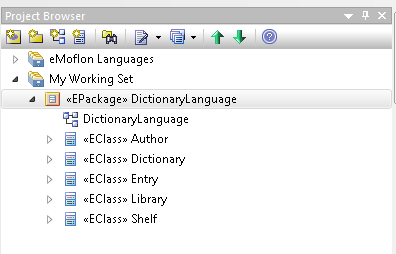
\includegraphics[width=0.4\textwidth]{ea_dictLangProBrowser}
  \caption{The \texttt{DictionaryLanguage} metamodel structure}
  \label{fig:dictionaryLangStart}
\end{center}
\end{figure}

\item[$\blacktriangleright$] It should be said that while you are able to copy and paste packages between multiple EAPs (i.e., copy
\texttt{<<EPack\-age>>DictionaryLanguage} into the \texttt{MyWorkingSet} root note of your source metamodel), if any of the copied packages have dependencies on
other packages, it cannot be done so easily. All links would be destroyed! If you tried to copy \texttt{DictionaryLanguage}, for example, the receiving project
would not be able to establish the necessary links to eMoflon's \texttt{Moca Language}.

\clearpage

\item[$\blacktriangleright$] Therefore, to properly migrate packages, you have to export a \emph{complete} node to an XMI file. To do this, right-click on the
\texttt{<<EPack\-age>>DictionaryLanguage} and navigate to ``Import/Export" and select \texttt{Export Model to XMI\ldots} (Fig.~\ref{fig:contextExport}).
Alternatively, you can select the root in the project browser and press \texttt{Ctrl + Alt + E}.

\vspace{0.5cm}

\begin{figure}[htbp]
\begin{center}
  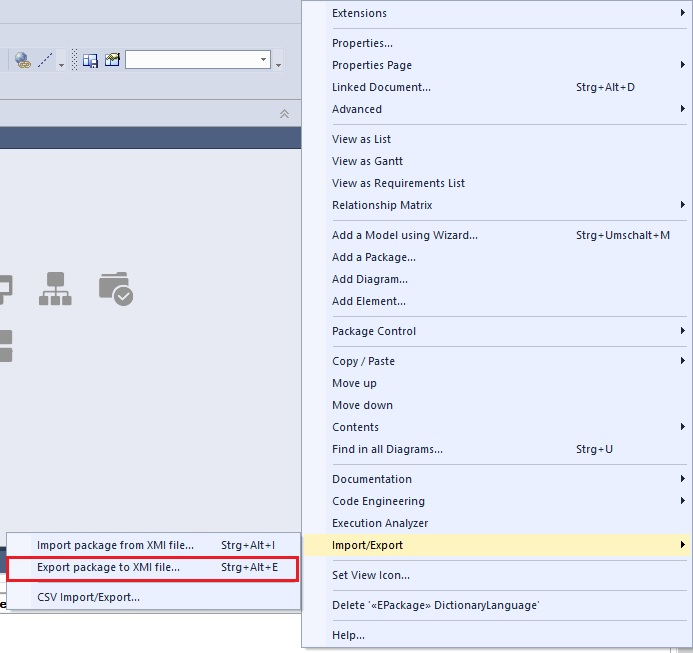
\includegraphics[width=\textwidth]{ea_contextExport}
  \caption{Starting the export process in EA}
  \label{fig:contextExport}
\end{center}
\end{figure}

\item[$\blacktriangleright$] Change the export type to \texttt{XMI 2.1} and save the file somewhere easily accessible (such as your desktop). Press export, and
close the window once the small green bar appears (Fig.~\ref{fig:export}).

\vspace{0.5cm}

\begin{figure}[htbp]
\begin{center}
  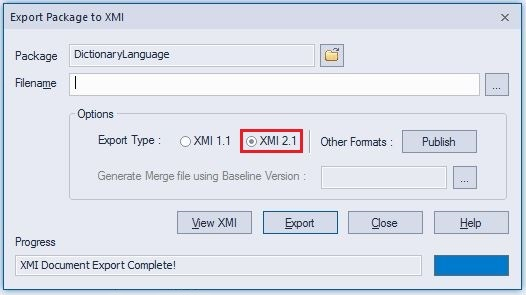
\includegraphics[width=0.9\textwidth]{ea_dialogueExport}
  \caption{Exporting the metamodel to a file}
  \label{fig:export}
\end{center}
\end{figure}

\item[$\blacktriangleright$] Open \texttt{LeitnersLearningBox.eap} from your Eclipse workspace and right-click anywhere in the project browser. Navigate to
``Import Model from XMI\ldots''

\item[$\blacktriangleright$] Find the \texttt{.xmi} file you just saved and press \texttt{import}. Press \texttt{OK} in the confirmation dialogue; Your project
browser should now resemble Fig.~\ref{fig:importProBrowser}.

\begin{figure}[htbp]
\begin{center}
  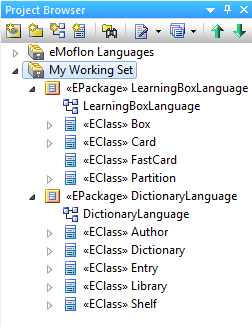
\includegraphics[width=0.4\textwidth]{ea_importedProjectBrowser}
  \caption{The TGG metamodels successfully included in one project}
  \label{fig:importProBrowser}
\end{center}
\end{figure}

\clearpage

\item[$\blacktriangleright$] Confirm everything worked by validating and exporting the dual-metamodel project to Eclipse, refreshing the package explorer to
build your workspace. You can do this with the eMolfon control panel, pressing \texttt{All} under \texttt{Validate}.\footnote{To review the details of how to
use the eMoflon control panel, read Section 2.8 from Part II}

\item[$\blacktriangleright$] After the validation completes, switch back to Eclipse and refresh your package explorer by pressing \texttt{F5}. A new
\texttt{DictionaryLanguage} project should have appeared under \texttt{My Working Set}.

\item[$\blacktriangleright$] That's everything! You're now ready to start your first transformation using your source and target metamodels.

\jumpSingle{TGGSchema}

\end{itemize}
